\documentclass{article}

\usepackage{arxiv}
\usepackage[utf8]{inputenc} % allow utf-8 input
\usepackage[T1]{fontenc}    % use 8-bit T1 fonts
\usepackage{hyperref}       % hyperlinks
\usepackage{url}            % simple URL typesetting
\usepackage{booktabs}       % professional-quality tables
\usepackage{amsfonts}       % blackboard math symbols
\usepackage{nicefrac}       % compact symbols for 1/2, etc.
\usepackage{microtype}      % microtypography
\usepackage{amsmath}
\usepackage{lipsum}
\usepackage{caption}
\usepackage{float}
\usepackage{graphicx}
\usepackage{subcaption}

% the comment 'DATA POINT' will mark where data was calculated and then inserted into
% the paper.

\newcommand{\der}[2][t]{\frac{\mathrm{d}#2}{\mathrm{d}#1}}

\title{Time Series Analysis of Chaotic Dynamical Systems with Recurrent Neural Networks}

\author{
  Lucas Wilson \\
  Undergraduate: Mathematics, Computer Science \\
  Colorado State University\\
  Fort Collins, CO 80523 \\
  \texttt{lkwilson96@gmail.com} \\
}

\begin{document}
\maketitle

\begin{abstract}
This is a paper about chaos.
\end{abstract}

%%% INTRODUCTION %%%
\section{Introduction}

This is a paper about chaos.
% TODO: mention \texttt{echonn}

%%% CHAOS %%%
\section{Chaos}

\subsection{History}

In 1963, Edward N. Lorenz published an article researching a simplified
system of ordinary differential equations modeling a convective system
\cite{lorenz1963deterministic}. His research popularized the possibility of a
system being highly sensitive to initial conditions, i.e., chaos theory;
while he wasn't the first to discover this phenomenon, he is considered to be
the "official discoverer of chaos theory" \cite{oestreicher2007history}.

When forecasting, the goal is to have accurate predictions. However, a
chaotic system's sensitivity to initial conditions implies that a small
perturbation as a result of error will produce incorrect solutions. Further,
given a periodic solution, the hope is that a small perturbation, from error
in measurement or from floating-point errors in numerical calculations,
doesn't affect the solution or at least produces a quasi-periodic solution
close to the periodic one. (A solution or trajectory $F$ is quasi-periodic if
and only if for all $t$ and for some $\tau$, $F(t+\tau)$ is arbitrarily close
to $F(t)$ \cite{lorenz1963deterministic}.)

An example of this is the trajectories of the sun and planets in our solar
system. Newton's equations can be used to create a system of equations to
model the bodies of mass (known as the n-body problem). However, with the
existence of other bodies of mass from other solar systems within the
universe, small perturbations are introduced into the system. If the system
is chaotic, then over time, the actual trajectories will diverge from our
model's \cite{oestreicher2007history}.

One of the defining characteristics of chaos is that the error from
perturbations grows exponentially \cite{oestreicher2007history}. At the time
of Lorenz's paper, unstable error was not well understood, and this led to
Lorenz's surprising discovery \cite{oestreicher2007history}. Lorenz reported
that a single iteration in calculating the solution to the dynamical system
took approximately one second \cite{lorenz1963deterministic}. In his paper,
he shows one of his calculations having about 3000 iterations, which must
have taken around 50 minutes. Given the amount of time it takes to perform
the calculation, it's tempting to continue the calculation from the output of
the previous calculation. However, the story of the discover is that while
the computer used 6 digit accuracy, it output only 3 digits, so when the
simulation was continued by Lorenz with the less accurate measurements, he
found the results to be very different \cite{oestreicher2007history}.

Chaos can appear in many different situations. Lorenz's paper demonstrates
chaos in a dynamical system useful for forecasting convection in the
atmosphere or liquids \cite{lorenz1963deterministic}. "Chaos theory has a few
applications for modeling endogenous biological rhythms such as heart rate,
brain functioning, and biological docks" \cite{oestreicher2007history}. It
can also appear in solutions to Hamiltonian problems such as the 3 body
problem (as mentioned before) and the double pendulum problem (as I will show
later). Understanding the predictability of chaos is very useful to many
different fields.

\subsection{Lyapunov Constant}

In terms of forecasting, it's useful to know how chaotic a dynamical system
is. Chaos will be measured by the exponential rate at which nearby
trajectories diverge. Constants describing the divergence are known as the
Lyapunov Characteristic Exponents (LCEs) \cite{sandri1996numerical}. There is
an LCE for each dimension, and since they all represent exponential growth.
The error growing at the rate of the largest LCE will dominate over the
others.

% TODO: talk about attractors

Given a small perturbation $\epsilon$ to a dynamical system in the direction
of the largest LCE, we can approximate the growth of the perturbation by the
equation $\epsilon(\Delta t) = \epsilon_0 e^{\lambda \Delta t}$ where
$\lambda$ is the largest LCE \cite{bezruchko2010extracting}. For an LCE of
zero, then the error doesn't grow exponentially, and thus, there is no chaos.
Error created from smaller LCEs is negligible. The approximate time scale
where perturbations become large is going to be proportional to $1 /
\lambda$. This is known as the Lyapunov time \cite{bezruchko2010extracting}.
For our solar system, the Lyapunov time is 10,000,000 years
\cite{oestreicher2007history}. Researchers have used it to evaluate the
effectiveness of forecasting models on chaotic problems
\cite{pathak2018model}. Predicting the solution of a chaotic model over an
interval of time which is multiple times the size of the Lyapunov time shows
the predictability of a model.

In order to find the Lyapunov time, we only need to solve for the largest
LCE. To find this, we will use a method detailed in
\cite{viswanath1998lyapunov}.

% TODO: Lyapunov calculation
% TODO: Test with Circle yielding zero

%%% DYNAMICAL SYSTEMS %%%
\section{Dynamical Systems}

Three dynamical systems will be used to demonstrate the predictability of
chaotic systems: the Lorenz system, Poincaré's 3-body problem solution, and
the double pendulum system. The Poincaré system is the one of the first, and
the Lorenz system is a classic example. The double pendulum is commonly
referred to as chaotic, and I will show this later. Both Poincaré's
restricted 3 body problem solution and the double pendulum are Hamiltonian
systems representing physical systems within our universe.

% TODO: numerical solutions section

\subsection{Lorenz System}

% TODO: Image of Lorenz System

The Lorenz system was originally based on a system of equations modeling
convection created by Saltzman \cite{lorenz1963deterministic}
\cite{saltzman1962finite}. Simplified by Lorenz, it is defined as follows
\cite{lorenz1963deterministic}:

\begin{align}
    \der{x} &= \sigma (y - x), \nonumber \\
    \der{y} &= x (\rho - z) - y, \nonumber \\
    \der{z} &= x y - \beta z. \label{eq:lorenz_equation}
\end{align}

Not all parameters for the Lorenz equation will produce chaotic behavior. In
Lorenz's article, he uses the parameter values $\sigma=10$, $\beta=8/3$, and
$\rho=28$ \cite{lorenz1963deterministic}, and it has a maximum LCE of
$0.90566$ \cite{viswanath1998lyapunov}. There are other parameters which
produce chaotic results outlined in Table \ref{table:lorenz_params}. Also
shown in Table \ref{table:lorenz_params} are the values calculated by my
Python module \texttt{echonn} are listed. These values are not as accurate,
but demonstrate the sufficient accuracy of \texttt{echonn}.

\begin{table}[H]
    \centering
    \begin{tabular}{|l|l|l|l|l|l|l|}
         % TODO: \lambda_1?
         % TODO: calculated values
        \hline
        $\sigma$ & $\rho$ & $\beta$ & actual $\lambda$ & calculated $\lambda$ & relative error of calculated $\lambda$ \\
        \hline \hline
        16 & 45.92 & 4 & 1.50255 & & \\ % DATA POINTS
        16 & 40 & 4 & 1.37446 & & \\
        10 & 28 & 8/3 & 0.90566 & & \\
        \hline
    \end{tabular}
    \caption{
        Lorenz Parameters and Largest Lyapunov Exponent
        \cite{viswanath1998lyapunov}
    }
    \label{table:lorenz_params}
\end{table}

\subsection{3-Body Problem}

The 3-body problem, or the generalized n-body problem, is a famous problem
which many have analyzed; most notably, Herni Poincaré wrote many papers
developing the area significantly \cite{chenciner2000remarkable}. One of
Poincaré's solutions, known as the circular restricted 3-body problem,
demonstrates chaotic properties \cite{oestreicher2007history}. Poincaré
performs several reductions of the original 3-body problem in order to come
to a much more useful form of the problem. The mass of one of the objects is
assumed to be negligible. This is the case for Sun-Earth-Moon orbits. The
moon has little effect on the orbit of the sun. Another aspect is the
rotating reference frame. Since the mass of one of the bodies is negligible,
the problem simplifies to first solving a two body problem. While much easier
to solver, Poincaré went further to stop the motion of the two planets by
using a rotating reference frame. Rotating with the planets, the problem can
be modeled seemingly by two static planets and a third mass-less planet
orbiting around those in a two dimensional plane.

% norm from https://tex.stackexchange.com/questions/107186/how-to-write-norm-which-adjusts-its-size
\newcommand{\norm}[1]{\left\lVert#1\right\rVert}
\newcommand{\rv}{\mathbf{r}}

The N body problem is defined as follows \cite{chenciner2000remarkable}:

Let $\rv_i$ be the position of the $i^\text{th}$ body in the N body problem.
Then, the force of gravity is the sum of gravity from every other body in the
system. That is,

\begin{equation}
   F_g^{(i)} = m_i \frac{\mathrm{d}^2 \rv_i}{\mathrm{dt}^2} =
   \sum_{j \neq i} G \frac{m_i m_j \hat{\rv}_{ij}}{\norm{\rv_{ij}}^3}
   \label{eq:nbody}
\end{equation}

where $\rv_{ij} = \rv_j - \rv_i$, $m_i$ is the mass of body $i$, and $G$ is
the gravitational constant.

For our purposes, the reduced system is more useful since it is much easier
to calculate than numerically solving the original 3-body problem. With three
bodies in three dimension, their motion is described by 9 second order
differential equations. Therefore, reducing the system to first order
differential equations yields 18 first order equations. The reduced problem
only requires 4 first order differential equations since the position is
defined by two second order differential equations.

Derived in \cite{eberle2007case}, the system of equations defined with
dimensionless rotating (synodic) coordinates:

\begin{align}
    x'' - 2 y' &= x
        - \frac{\alpha}{r_1^3} (x - \mu)
        - \frac{\mu}{r_2^3} (x + \alpha) \nonumber \\
    y'' + 2 x' &= \left(
        1 - \frac{\alpha}{r_1^3}
        - \frac{\mu}{r_2^3}
    \right) y \nonumber \\
\end{align}

where 

\begin{align}
    \mu &= \frac{m_1}{m_1 + m_2} \nonumber \\
    \alpha &= 1 - \mu \nonumber \\
    r_1(t) &= \left[(x(t) - \mu)^2 + y(t)^2\right]^{\frac{1}{2}} \nonumber \\
    r_2(t) &= \left[(x(t) + \alpha)^2 + y(t)^2\right]^{\frac{1}{2}} \label{eq:reduc_3body_cor}
\end{align}
 
and where mass body 1 and two are located at $-\alpha$ and $\mu$.

If we define the following system:

\begin{align}
    x_1 &= x \nonumber \\
    x_2 &= x' \nonumber \\
    y_1 &= y \nonumber \\
    y_2 &= y', \label{eq:first_order_def}
\end{align}

then, we can take the derivative of each:

\begin{align*}
    x_1' &= x' \\
    &= x_2,
\end{align*}
and
\begin{align*}
    x_2' &= x'' \\
    &= 2 y' + x
        - \frac{\alpha}{r_1^3} (x - \mu)
        - \frac{\mu}{r_2^3} (x + \alpha) \\
    &= 2 y_2 + x_1 - \frac{\alpha}{r_1^3} (x_1 - \mu)
        - \frac{\mu}{r_2^3} (x_1 + \alpha),
\end{align*}
and
\begin{align*}
    y_1' &= y' \\
    &= y_2,
\end{align*}
and
\begin{align*}
    y_2' &= y'' \\
    &= - 2 x' + \left(
        1 - \frac{\alpha}{r_1^3}
        - \frac{\mu}{r_2^3}
    \right) y \\
    &= - 2 x_2 + \left(
        1 - \frac{\alpha}{r_1^3}
        - \frac{\mu}{r_2^3}
    \right) y_1.
\end{align*}

Then, we can represent the second order system of motion as four first order
equations:

\begin{align}
    x_1' &= x_2 \nonumber \\
    x_2' &= 2 y_2 + x_1 - \frac{\alpha}{r_1^3} (x_1 - \mu)
        - \frac{\mu}{r_2^3} (x_1 + \alpha) \nonumber \\
    y_1' &= y_2 \nonumber \\
    y_2' &= - 2 x_2 + \left(
        1 - \frac{\alpha}{r_1^3}
        - \frac{\mu}{r_2^3}
    \right) y_1, \label{eq:reduce_3_body_prog_sys} \\
\end{align}

where 

\begin{align}
    r_1 &= \left[(x_1 - \mu)^2 + y_1^2\right]^{\frac{1}{2}} \nonumber \\
    r_2 &= \left[(x_1 + \alpha)^2 + y_1^2\right]^{\frac{1}{2}}.
\end{align}

Here, $x_1$ and $y_1$ represent the position of the third body relative to
the other two, but not in the standard Cartesian coordinates of 3D space.
Outlined in the paper \cite{eberle2007case}, the transformation back to
Cartesian coordinates is given, but we don't need the exact position of the
bodies since we are only concerned with the chaotic motion, so that isn't
shown here.

There are however two issues when integrating this problem. As objects
approach each other, the distance between them approaches zero. If collision
occurs, then this approaches infinity. There is no collision detection in
this model, and each body has a radius of zero, so this case is not handled.
Instead, a divide by zero error occurs, and the model cannot be calculated
further.

Further, near collisions are also an issue. With the distance between bodies
approaching zero, their potential energy becomes significantly smaller than
other values, such as those describing kinetic energy
\cite{chambers1999hybrid}. This produces a stiff system of equations, and
introduces error. Since energy is conserved in this Hamiltonian system, the
error introduced represents energy being created. This can cause the
singularity property seen in Figure \ref{fig:singularity}. This problem can
be solved by using a symplectic integrator \cite{chambers1999hybrid}.

\begin{figure}[H]
    \centering
    \begin{subfigure}[b]{0.3\textwidth}
        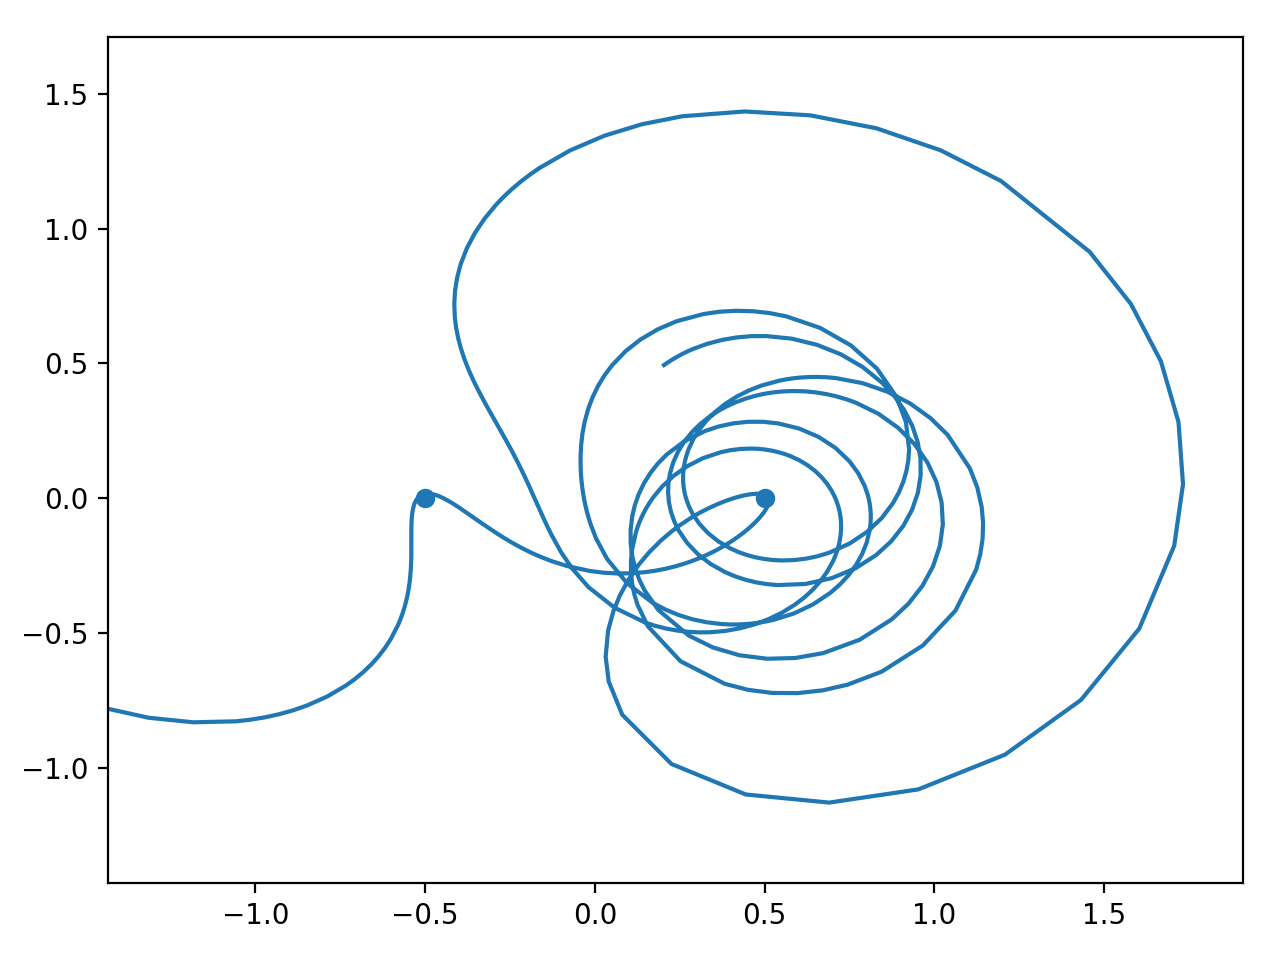
\includegraphics[width=\textwidth]{images/r3b_collision.png}
        \caption{The restricted 3 body problem with collision}
        \label{fig:r3b_collision}
    \end{subfigure}
    ~
    \begin{subfigure}[b]{0.3\textwidth}
        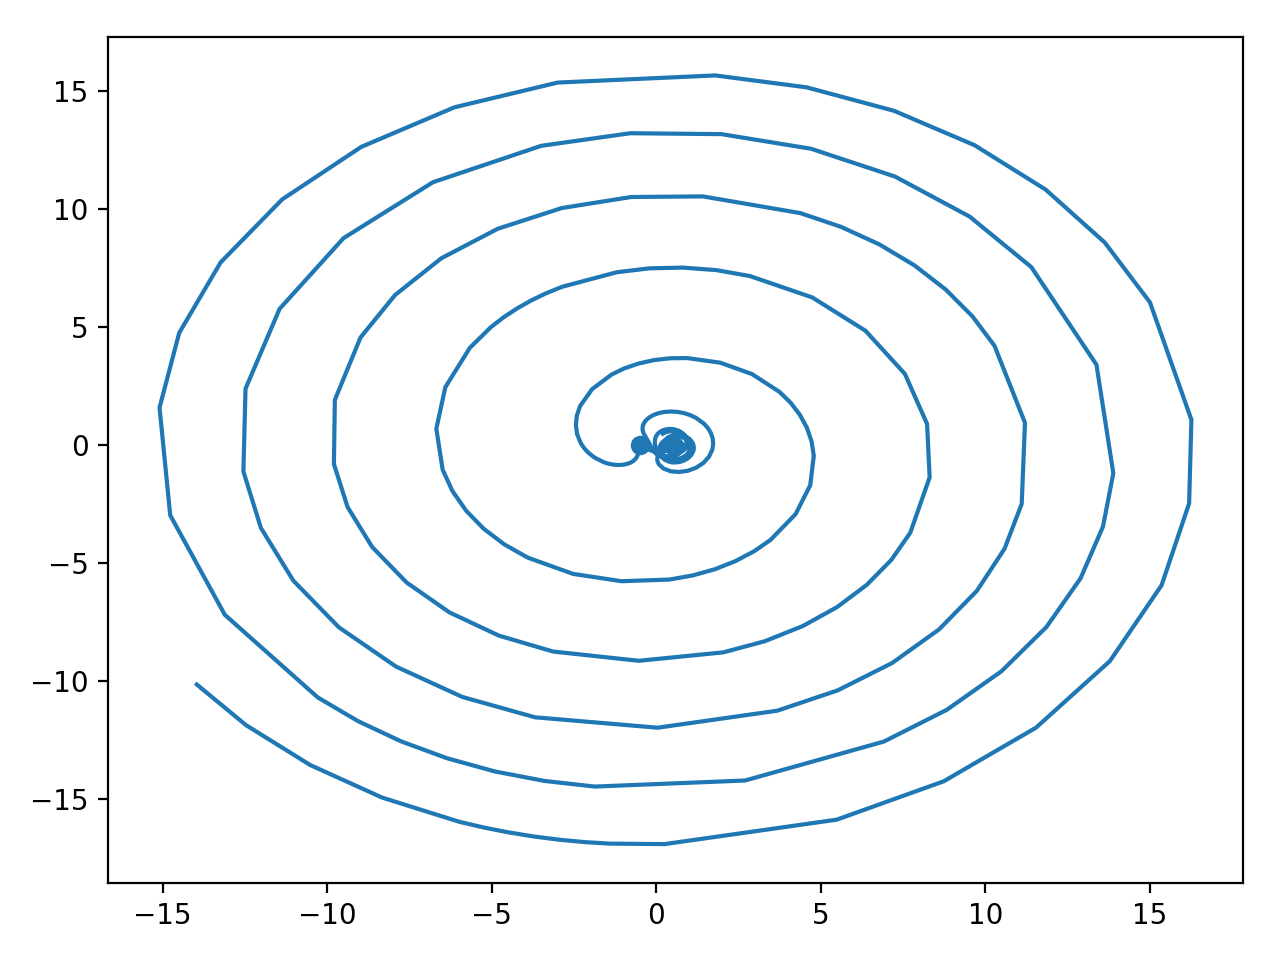
\includegraphics[width=\textwidth]{images/r3b_collision_whole.png}
        \caption{The resultant divergence of the body}
        \label{fig:r3b_collision_whole}
    \end{subfigure}
    \caption{The Restricted 3 Body Problem Error from Collision}
    \label{fig:singularity}
\end{figure}

While it is possible to use a symplectic integrator, it is not necessary.
Under the right initial conditions, the third body will diverge regardless.
The simple divergent spiral isn't chaotic, so instead orbital and collision
less initial conditions will be used. Without divergence and without
collisions, the symplectic integrator is unnecessary.

\subsection{Double Pendulum}

The double pendulum is commonly cited to be chaotic
\cite{stachowiak2006numerical} \cite{levien1993double}. Using the system of
equations derived by Stachowiak \cite{stachowiak2006numerical}, the system is
defined as follows:

\begin{align}
    \der{\theta_1} &= \omega_1, \nonumber \\
    \der{\theta_2} &= \omega_2, \nonumber \\
    \der{\omega_1} &= 
    \frac{
        \sin(\theta_1 - \theta_2) \lbrack
            l_1 \cos(\theta_1 - \theta_2) \omega_1^2 + \omega_2^2
        \rbrack
    }{
        2 l_1 \lbrack
            1 + m_1 - \cos^2(\theta_1 - \theta_2)
        \rbrack
    }
    -
    \frac{
        (1 + 2 m_1) \sin \theta_1 + \sin(\theta_1 - 2 \theta_2)
    }{
        l_1 \lbrack
            1 + m_1 - \cos^2(\theta_1 - \theta_2)
        \rbrack
    }
    , \nonumber \\
    \der{\omega_2} &= \sin (\theta_1 - \theta_2) 
    \frac{
        (1+m_1) (\cos \theta_1 + l_1 \omega_1^2)
        +
        \cos(\theta_1 - \theta_2) \omega_2^2
    }{
        1 + m_1 - \cos^2(\theta_1 - \theta_2)
    }. \label{eq:doub_pen}
\end{align}

$\theta_1$ and $\omega_1$ represent the angle and angular velocity of the
inner pendulum where $\theta_1=0$ implies the pendulum is straight down, and
$\theta_1=\epsilon$ implies the pendulum is rotated $\epsilon$ radians
counter-clockwise. The same is true for the outer pendulum relative to its
pivot point, the end of the first pendulum. $l_1$ and $l_2$ are the lengths
of the inner and outer pendulums, respectively. $m_1$ and $m_2$ are the
masses of the balls on the end points of the inner and outer pendulums,
respectively. Then, the positions of the endpoints $(x_1$, $y_1)$ and $(x_2,
y_2)$ of the pendulum, with the center pivot at the origin, $(0, 0)$, can be
calculated as follows:

\begin{align}
    x_1 &= l_1 \sin(\theta_1), \nonumber \\
    y_1 &= - l_1 \cos(\theta_1), \nonumber \\
    x_2 &= x_1 + l_2 \sin(\theta_2), \nonumber \\
    y_2 &= y_1 - l_2 \cos(\theta_2), \label{eq:doub_pend_endpoints}
\end{align}

\begin{figure}[H]
    \centering
    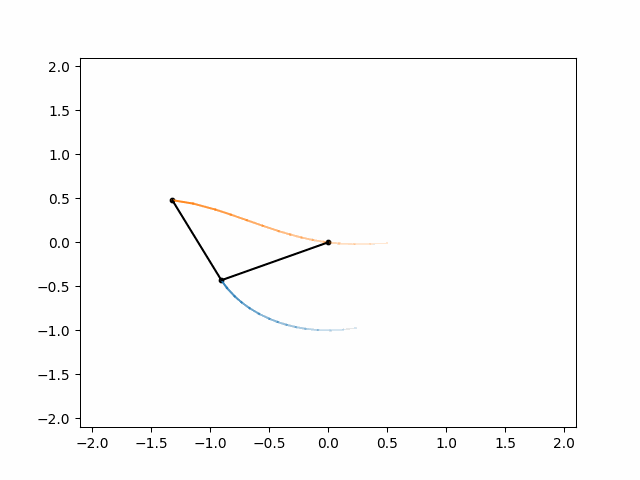
\includegraphics[width=.5\linewidth]{images/example_doub_pend.png}
    \caption{The Double Pendulum}
    \label{fig:doub_pend}
\end{figure}

% TODO: position of the pendulum end points

While the system is a Hamiltonian system, Stachowiak decided to define the
first order derivative components as angular velocity as opposed to momentum.
This won't affect anything regarding the purpose of this paper.

Interestingly, the degree of chaos is dependent on the initial conditions
\cite{levien1993double}. In the experiment, the initial conditions had
angular velocities of zero, the outer pendulum was straight down, and the
inner pendulum varied from 0 degrees to 180 degrees \cite{levien1993double};
the results showed that the LCE increased with theta.

Repeating the same experiment, but with different parameters ($l_1 = l_2 =
1$, and $m_1 = m_2 = 1$), the results are similar (see Figure
\ref{fig:doub_pend_energy}). As inner theta increases, the largest LCE of the
system seems to approach 1.4. % DATA POINT

\begin{figure}[H]
    \centering
    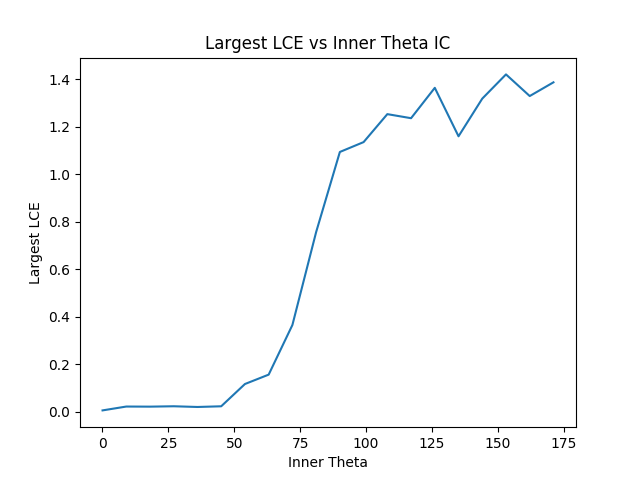
\includegraphics[width=.5\linewidth]{images/chaos_vs_energy_in_doub_pend.png}
    \caption{Largest Lyapunov Characteristic Exponent vs Inner Theta Initial Condition}
    \label{fig:doub_pend_energy}
\end{figure}

%%% MODELS %%%
\section{Models}

\subsection{ARIMA}
%\subsection{Recurrent Neural Networks}
\subsection{Echo State Networks}
%\subsection{LTSM}

%%% ANALYSIS %%%
\section{Analysis}

\subsection{Method}
\subsection{Results}

%% CONCLUSION %%%
\section{Conclusion}

\bibliography{references}
\bibliographystyle{unsrt}

\end{document}

% Useful LaTeX commands

%\section{Headings: first level}
%\subsection{Headings: second level}
%\subsubsection{Headings: third level}

%\keywords{First keyword \and Second keyword \and More}

% \paragraph{Paragraph}

%% \begin{figure}
%%   \centering
%%   \fbox{\rule[-.5cm]{4cm}{4cm} \rule[-.5cm]{4cm}{0cm}}
%%   \caption{Sample figure caption.}
%%   \label{fig:fig1}
%% \end{figure}

%%\author{
  %%Lucas Wilson \\
  %%Undergraduate: Mathematics, Computer Science \\
  %%Colorado State University\\
  %%Fort Collins, CO 80523 \\
  %%\texttt{lkwilson96@gmail.com} \\
  %% \AND
  %% Coauthor \\
  %% Affiliation \\
  %% Address \\
  %% \texttt{email} \\
  %% \And
  %% Coauthor \\
  %% Affiliation \\
  %% Address \\
  %% \texttt{email} \\
  %% \And
  %% Coauthor \\
  %% Affiliation \\
  %% Address \\
  %% \texttt{email} \\
%%}
